\section{多様体}
多様体には第二可算性を課す。

\subsection{はめ込まれた部分多様体}
記法がややクソかもしれない。
\begin{rem}[記法]
    多様体は$M,N$、(はめ込まれた)部分多様体は$\iota:P\hookrightarrow M$、$C^\infty$級写像は$\phi,\psi:M\to N$、$C^\infty$級関数は$f,g:M\to\R$。近傍はどの点の周りかを表して$U_p,U_q$などと書く。局所座標は$\tau,\sigma:U\to\R^n$などを使い、簡単のため像は常に$\R^d$全体とする。
\end{rem}
逆関数定理はあればあるほど良い。
\begin{rem}[逆関数定理]
    多様体$M,N$とその間の$C^\infty$級写像$\phi:M\to N$と$p\in M,\ q:=\phi(p)$について
    \begin{enumerate}[(1)]
        \item 微分$d\phi_p:T_pM\to T_qN$が単射なら、ある局所座標$(U_p,\tau),(U_q,\sigma)$が存在し
        \[\R^d\xrightarrow[\tau^{-1}]{\cong} U_p\xrightarrow{\phi}U_q\xrightarrow[\sigma]{\cong}\R^c\ =\ \R^d\hookrightarrow\R^c\]
        とできる。ここで、$\R^d\hookrightarrow\R^c$とは標準的な包含写像である。
        \item 微分$d\phi_p:T_pM\to T_qN$が全射なら、ある局所座標$(U_p,\tau),(U_q,\sigma)$が存在し
        \[\R^d\xrightarrow[\tau^{-1}]{\cong} U_p\xrightarrow{\phi}U_q\xrightarrow[\sigma]{\cong}\R^c\ =\ \R^d\twoheadrightarrow\R^c\]
        とできる。ここで、$\R^d\twoheadrightarrow\R^c$とは標準的な全射である。
    \end{enumerate}
    つまり、局所的には自明な線形写像にできる、ということである。
\end{rem}


\begin{rem}[部分多様体]
    はめ込まれた部分多様体を単に「部分多様体」と呼ぶ。つまり、$\iota:P\hookrightarrow M$について
    \begin{center}
        はめ込み$\Leftarrow$単射なはめ込み$\Leftarrow$埋め込み
    \end{center}
    という論理包含があるが、この真ん中を満たす$\iota$を部分多様体と呼ぶ。恐らく、埋め込みを部分多様体と呼ぶのが平均的な定義だと思うが、わざわざそれよりも弱い定義を採用するのは理由がある。後述するFrobeniusの定理によって自然に表れる極大積分多様体という対象は埋め込みにならないからである。
\end{rem}
はめ込みは各点の微分が単射であることで、埋め込みは像への同相を誘導するはめ込みであった。しかし、これだけだとあまり思い出せた気がしないので簡単な例を軽く紹介する。
\begin{eg}[not はめ込み]
    $\iota:\R\ni x\longmapsto x^3\in\R$ という写像ははめ込みでない。しかし同相ではある。
\end{eg}
\begin{eg}[はめ込み but not 部分多様体]
    自己交叉するものは全てこれである。矢印は曲線の向きを表す。
    \[\begin{tikzpicture}
        \draw (1,1) to [out=-135,in=-90] (-2,0);
        \draw[->] (-2,0) to [out=90,in=135] (1,-1);
    \end{tikzpicture}\]
\end{eg}
\begin{eg}[部分多様体 but not 埋め込み]
これが一番重要である。前者は悪いが後者は良い部分多様体である。
    \begin{itemize}
        \item 8の字のやつ(どちらも$\R$からの像であって$\to\pm\infty$で原点に近づくが、近づく方向が違う)
        \[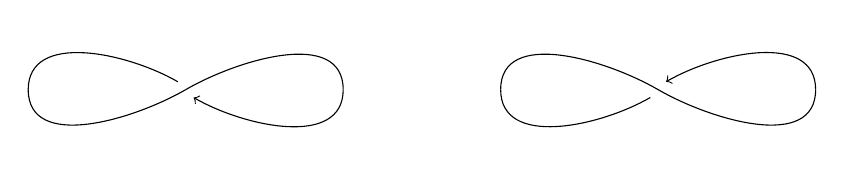
\begin{tikzpicture}
            \draw (-3-0.1,0.1) to [out=150,in=90] (-3-2,0);
            \draw (-3-2,0) to [out=-90,in=-150] (-3,0);
            \draw (-3,0) to [out=30,in=90] (-3+2,0);
            \draw[->] (-3+2,0) to [out=-90,in=-30] (-3+0.1,-0.1);
            
            \draw (3-0.1,-0.1) to [out=-150,in=-90] (3-2,0);
            \draw (3-2,0) to [out=90,in=150] (3,0);
            \draw (3,0) to [out=-30,in=-90] (3+2,0);
            \draw[->] (3+2,0) to [out=90,in=30] (3+0.1,0.1);
        \end{tikzpicture}\]
        \item トーラスにめっちゃ巻き付くやつ。$\iota:\R\ni t\longmapsto(\exp(2ti),\exp(2\alpha ti))\in \T^2$ を$\alpha\in\R\setminus\Q$について考えると、稠密になって滅茶苦茶な絵になる。
        \[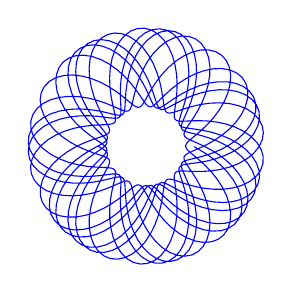
\begin{tikzpicture}
            \draw[blue,samples=1000,domain=-9*pi:10*pi,variable=\theta] plot(\theta r:{0.5+sin(1.79*\theta r)^2});
            
        \end{tikzpicture}\]
    \end{itemize}
    後者の良い部分多様体に主に興味がある。これは$X:=\pdiff{}{\theta_1}+\alpha\pdiff{}{\theta_2}$というベクトル場の積分曲線であるが、Frobeniusの定理は積分曲線の次元を上げた(つまり$c$個のベクトル場を積分してできる$c$次元の部分多様体)についての定理である。
\end{eg}
部分多様体$\iota:P\hookrightarrow M$は単射だから、$\iota$とは$M$の部分集合$P$上での多様体構造のことと言ってもよい。「$P\subset M$がはめ込まれた部分多様体」という言明は$P$上の位相とか微分構造を指定しないと意味をなさない一方、「$P\subset M$が埋め込まれた部分多様体」という言明は意味をなす。
\begin{rem}[埋め込みの特徴付け]
    $P\subset M$が埋め込み$\iff$局所的に$(P,M)$は$(\R^c,\R^d)$に微分同相。\\
    つまり、$\forall p\in P\ \exists(U_p,\tau)\ \tau(U_p\cap P)=\R^c\times\{0\}$ となること。
\end{rem}
\begin{eg}[複数の位相が入る部分多様体]
    $M:=\R^2,\ P$を8の字とする。図のように二通り$\R$からの$C^\infty$像だと思える
    \[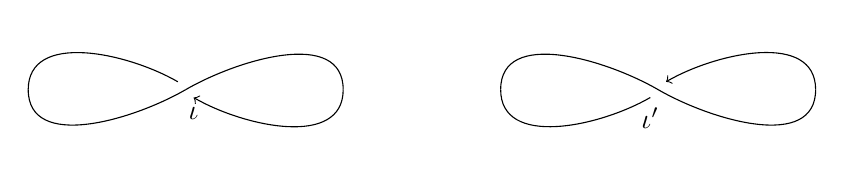
\begin{tikzpicture}
        \draw (-3-0.1,0.1) to [out=150,in=90] (-3-2,0);
        \draw (-3-2,0) to [out=-90,in=-150] (-3,0);
        \draw (-3,0) to [out=30,in=90] (-3+2,0);
        \draw[->] (-3+2,0) to [out=-90,in=-30] (-3+0.1,-0.1)node[below]{$\iota$};
        
        \draw (3-0.1,-0.1)node[below]{$\iota'$} to [out=-150,in=-90] (3-2,0);
        \draw (3-2,0) to [out=90,in=150] (3,0);
        \draw (3,0) to [out=-30,in=-90] (3+2,0);
        \draw[->] (3+2,0) to [out=90,in=30] (3+0.1,0.1);
    \end{tikzpicture}\]
    が、$\iota'=\iota\circ\text{hoge}$となる$\R$の微分同相hogeは存在しない。
    \[\begin{tikzcd}
        \R\arrow[dr,"\not\exists\ \text{hoge}"'] \arrow[r,"\iota'"] & \R^2\\
	&	\R\arrow[u,"\iota"]
    \end{tikzcd}\]
\end{eg}
しかし、実は次が成立する。
\begin{prop}\label{prop:111}
	\begin{enumerate}[(a)]
		\item $P(\subset M)$上の位相を一つ固定する。この位相と整合する$C^\infty$構造であって、$P\hookrightarrow M$が部分多様体となるようなものは高々一意である。
		\item $P(\subset M)$が埋め込みであるとする。このとき$P$を部分多様体とする$P$上の多様体としての構造(位相も取り換えて良い)は、$M$の微分構造から誘導されるもの($P$を埋め込みとするもの)だけである。
	\end{enumerate}
	つまり、部分多様体$P\subset M$とは本来「$P$と$P$の位相、$P$の微分構造」を指定しなければいけないところを、「$P$と$P$の位相」だけを指定すれば十分ということである。更に、埋め込まれた部分多様体は埋め込まれていない部分多様体になりえないのである。
\end{prop}
これを示す前に、準備として次の定理を証明する。
\begin{thm}
	部分多様体$\iota:P\hookrightarrow M$と$C^\infty$級写像$\phi:N\to M$に対し$\phi(N)\subset\iota(P)$となっていたとする。
	\[\begin{tikzcd}
	    N\arrow[r,"\phi"]\arrow[dr,"\phi_0"'] &M\\
	    & P\arrow[u,hook,"\iota"']
	\end{tikzcd}\]
	\begin{enumerate}[(a)]
	    \item $\phi_0$が連続$\Rightarrow \phi_0$が$C^\infty$級
	    \item $\iota:P\hookrightarrow M$が埋め込み$\Rightarrow \phi_0$は連続
	\end{enumerate}
\end{thm}
特に、埋め込みの場合は自動的に$\phi_0$は滑らかである。
\begin{proof}
    (b)は相対位相の普遍性である。(a)を示す。\\
    $n\in N$を取り、$p:=\phi_0(n),\ m:=\iota(p)$とし、近傍$U_n,U_p,U_m$を十分小さく取って$U_m\subset \iota(U_p),\ U_p\subset \phi_0(U_n)$とできる。$d\iota_p$は単射だから、逆関数定理より次を満たす$r:U_m\to P$が取れる。
    \[U_p\overset{\iota}{\longrightarrow}U_m\overset{r}{\longrightarrow}P\ =\ U_p\hookrightarrow P\]
    つまり、標準的な包含$\R^d\hookrightarrow\R^c$が左逆写像を持つことから、それの両側に微分同相を掛けた$\iota\lvert_U$も左逆写像を持つことになる、ということである。このような$r$の作り方から$r$は$C^\infty$級であり、$\phi_0$も$C^\infty$級。
    \[\phi_0\lvert_{U_n}=r\circ\iota\circ \phi_0\lvert_{U_n}=r\circ \phi\lvert_{U_n}\]
\end{proof}
\begin{proof}[Proof of 命題\ref{prop:111}]
    (a)は上の定理の(a)からすぐに従う。与えられた$P$上の位相と整合的な極大アトラス$\A_1,\A_2$に対し、$N,P$を$(P,\A_1),(P,\A_2)$とすれば $\id_P$が$C^\infty$となる。
    \[\begin{tikzcd}
        (P,\A_1)\arrow[r,hook]\arrow[dr,"\id"'] &M\\
	    & (P,\A_2)\arrow[u,hook]
    \end{tikzcd}\]
    $\A_1,\A_2$を入れ替えたら$\id_P$が微分同相になり、つまり$\A_1=\A_2$となる。\\
    (b)を示す。$P$上の多様体構造$(P,\O,\A)$であって包含写像$P\hookrightarrow M$が部分多様体になるものを取る。上の定理の(b)から$\id:(P,\O,\A)\to P$は$C^\infty$級になる。可読性のため、$\id=:\phi$と置く。
    \[\begin{tikzcd}
        (P,\O,\A)\arrow[r,hook]\arrow[dr,"\phi"'] &M\\
	    & P\arrow[u,hook]
    \end{tikzcd}\]
    この図式を微分に落とすと、部分多様体からの包含写像の微分は単射であり、可換性から$d\phi$は単射。
    \[\begin{tikzcd}
        (P,\O,\A)_p\arrow[r,hook]\arrow[dr,"d\phi"'] &M_p\\
	    & P_p\arrow[u]
    \end{tikzcd}\]
    今$f:(P,\O,\A)\to P$は全単射で微分が各点で単射。より一般にこういう状況においては、第二可算性から$\phi$の微分同相性が出てくる\footnote{第二可算性を課さない場合、連続体濃度の集合に離散位相を入れた0次元多様体は$\R$への全単射なはめ込みを持つ。}。なぜなら、$\phi:M\to N$について$M$の方が真に$N$より次元が低ければ像は$N$内で測度零になる。一方、次元が等しければ、微分$d\phi$は同じ次元の間の線形単射であり線形同型となる。
\end{proof}
\begin{defi}[スライス]
    $(U,\tau)$を$M$の局所座標とする。$\tau=(x_1,\dots,x_d)$と成分表示する($x_i:M\to\R$)。\\
    各$a\in\R^{d-c}$について
    \[S_a:=\tau^{-1}(\R^c\times\{a\})=\{(x_{c+1},\dots,x_d)=a\}\]
    という形の$U$の部分集合をスライスと呼ぶ。
\end{defi}
\begin{prop}[はめ込みは局所的にスライス]\label{prop:112}
    はめ込み$\iota:P\to M$について、各$p\in P$の近傍$U_p$で$\iota:U_p\to\iota(U_p)$が微分同相になるものが取れる。つまり、部分多様体は幾つかのスライスの和集合で書け、それらをアトラスとするようにできる。
\end{prop}
しかし、8の字の部分多様体を思い出すと分かる通り、$\iota(P)$に含まれるスライスが全て$P$の開集合になるとは限らない。
\begin{proof}
    逆関数定理から即座に従う。
\end{proof}
\begin{thm}[正則値定理]
    $\phi:M\to N$と部分多様体$\iota:Q\hookrightarrow N$に対し、$P:=\phi^{-1}(\iota(Q))$と置く。
    \[\begin{tikzcd}
        M\arrow[r,"\phi"] &N\\
        P\arrow[u,hook]\arrow[r,"\phi"] &Q\arrow[u,hook,"\iota"']
    \end{tikzcd}\]
    $\forall p\in P\ N_{\phi(p)}=d\phi(M_p)+d\iota(Q_{\phi(p)})$ のとき、$P$には自然に多様体構造が入り、$P\hookrightarrow M$は部分多様体、$\phi:P\to Q$は$C^\infty$級になる。更に、$Q\subset N$が埋め込みのとき$P\subset M$も埋め込みになる。
\end{thm}
これの$Q$が一点の場合がよく知られた正則値定理(このpdfだと単に逆関数定理と呼んでいるが)である。
\begin{proof}
    $P:=\set{(m,q)\in M\times Q}{\phi(m)=\iota(q)}$ と置く。つまり、これと$\phi^{-1}(\iota(Q))$に自然な全単射($M$成分だけから復元できる)があるが、$P$の多様体としての構造を$M\times Q$から誘導させる。という操作が許されるのは$P\subset M\times Q$が埋め込みになっている場合くらいだが、ちゃんとそれが成り立つことが確認できる。\\
    局所的に$P\subset M\times Q$が線形空間の自明な包含に微分同相であることを示せばいいから、$M,Q,N$は全てユークリッド空間$M=\R^a,Q=\R^b,N=\R^c$として良い。このとき$P$は次の写像の$\{0\}$の逆像。
    \[F:M\times Q=\R^a\times\R^b\ni(m,q)\longmapsto \phi(m)-\iota(q)\in\R^c=N\]
    各$P$の点でのこれの微分が全射になることが仮定だったから、逆関数定理より$F$は全射線形写像にとしてよい。つまり、座標を取れば$P=\ker F\subset M\times Q$という線形空間の包含にできるからOK。\\
    $P$から$M,Q$への写像は成分への射影で得られる。$P\hookrightarrow M$が部分多様体になることとかは微分の計算からすぐ出てくる。$Q\subset N$が埋め込みのとき$M\times Q\subset M\times N$も埋め込みだから$P\subset M\times N$も埋め込みになる。この$P$は次の$M'\subset M\times N$に含まれる。
    \[M':=\set{(m,n)\in M\times N}{f(m)=n}\]
    故に$P\subset M'$も埋め込みになるが、$M'$は$M$に微分同相である。
\end{proof}


\ \\
\subsection{Frobeniusの定理}
\begin{rem}[積分曲線]
    ベクトル場$X$の積分曲線$\gamma:(-\epsilon,\epsilon)\to M$とは
    \[\Dot{\gamma}(t)=X_{\gamma(t)}\]
    となるもののこと。$M$の各点に対しそこを通る積分曲線が存在し一意、という事実は常微分方程式論の基本的な結果から分かる。
\end{rem}
こういう感じのやつの高次元版が積分多様体である。つまり、$c$個のベクトル場が与えられたらそれらを「積分」してできる部分多様体が存在したり存在しなかったりするのである。ただ、$c$個のベクトル場$X_1,\dots,X_c$として扱うのではなく、$D_x:=\spn\{(X_1)_x,\dots,(X_c)_x\}$という「接空間の部分空間を滑らかに動かしたもの」として扱う。
\begin{defi}[分布]
    $D$が$M$上の$c$次元の分布であるとは、$\displaystyle D\subset TM,\ D=\bigcup_{x\in M}D_x,\ D_x\subset M_x$であって、$D_x\subset M_x$が$c$次元の部分空間であり$D_x$が$x$に関し$C^\infty$級に動くことを言う。\\
    ここで言う「$C^\infty$級」とは、局所的に$D$は$M$からGrassman多様体$\mathrm{Grass}(c,d)$への写像だと思ってその写像が$C^\infty$級という条件と見てもいいし、局所的にベクトル場$X_1,\dots,X_c$があって$\{(X_1)_x,\dots,(X_c)_x\}$が$D_x$の基底になるという条件と思ってもいい。
\end{defi}
\begin{defi}[積分多様体]
    $\iota:P\hookrightarrow M$が分布$D$の積分多様体であるとは、$\forall p\in P$に対し次を満たすこと。
    \[d\iota_p(P_p)=D_\iota(p)\]
\end{defi}
\begin{defi}[包合的]
    (良くない記法だが)分布$D$とベクトル場$X$に対し、$X$が$D$に属することを
    \[X\subset D\overset{def}{\iff}\forall x\in M\ X_m\in D_m\]
    と書く。このとき、$D$が包合的とは次を満たすこと。
    \[X,Y\subset D\Rightarrow [X,Y]\subset D\]
\end{defi}
\begin{rem}[基底だけ見ればいい]\label{rem:121}
    分布$D$は局所的には基底$\{X_1,\dots,X_c\}$を持つので、上の定義は次で言い換えられる。
    \[X\subset D\iff \exists a_1,\dots,a_c\text{:局所的に定義された関数}\ \ X=\sum_i a_iX_i\]
    \[D\text{が包合的}\iff \exists a_{i,j}^k\text{:局所的に定義された関数}\ \ [X_i,X_j]=\sum_k a_{i,j}^k X_k\]
\end{rem}
次が目標となる、Frobeniusの定理である。
\begin{thm}[Frobenius]\label{thm:121}
    分布$D$に対し「$\forall m\in M\ m$を通る積分多様体が存在」$\iff$「$D$が包合的」。
\end{thm}
よく分からない条件がよく分かる条件と同値なのは嬉しいが、直観が無いと辛いので絵を描く。
\[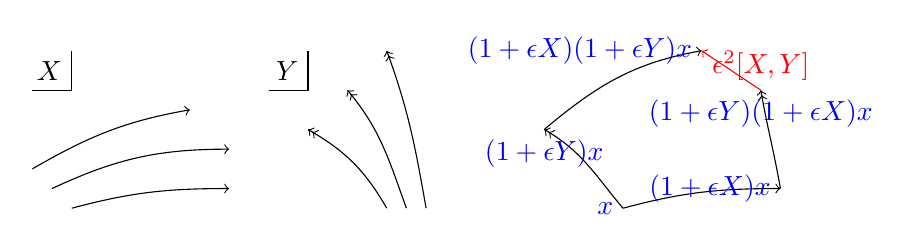
\begin{tikzpicture}
    \draw (0.5,1.5)--(1,1.5)node[above left]{$X$}--(1,2);
    
    \draw[->] (0.5,0.5) to [out=30,in=-170] (2.5,1.25);
    \draw[->] (0.75,0.25) to [out=25,in=-180] (3,0.75);
    \draw[->] (1,0) to [out=15,in=-180] (3,0.25);
    
    \draw (3.5,1.5)--(4,1.5)node[above left]{$Y$}--(4,2);
    
    \draw[<<-] (5,2) to [out=-70,in=100] (5.5,0);
    \draw[<<-] (4.5,1.5) to [out=-50,in=110] (5.25,0);
    \draw[<<-] (4,1) to [out=-30,in=120] (5,0);
    
    \draw[->>] (8,0)node[blue,left]{$x$} to [out=130,in=-30] (7,1)node[blue,below]{$(1+\epsilon Y)x$};
    \draw[->] (8,0) to [out=15,in=-180] (10,0.25)node[blue,left]{$(1+\epsilon X)x$};
    \draw[->>] (10,0.25) to [out=100,in=-80] (9.75,1.5)node[blue,below]{$(1+\epsilon Y)(1+\epsilon X)x$};
    \draw[->] (7,1) to [out=40,in=-170] (9,2)node[blue,left]{$(1+\epsilon X)(1+\epsilon Y)x$};
    \draw[red,->] (9.75,1.5)node[above]{$\epsilon^2[X,Y]$}--(9,2);
\end{tikzpicture}\]
まず、$[X,Y]$とは、$X,Y$の非可換性を表す量であった。時刻0で$x$を通る$X$の積分曲線の時刻$\epsilon$での点を$(1+\epsilon X)x$と書く(悪い書き方だが)と、$(1+\epsilon X)(1+\epsilon Y)x$と$(1+\epsilon Y)(1+\epsilon X)x$は一般には一致せず、その差がだいたい$\epsilon^2[X,Y]_x$くらいになる。\\
積分曲線とはベクトル場の矢印をなぞって曲線を描く操作だったのと同様、積分多様体とは$D_p$という微小な正方形をペタペタ貼り合わせていく操作となる。このとき貼り合わせていく順番が問題となる。\\
まず、$X\subset D$に対し$D_x$を$D_{(1+\epsilon X)x}$に動かす操作は「スライド」するだけで「上下方向のズレ」は生じない(これは$X_x\in D_x$だから)。つまり、$D_x$と$D_{(1+\epsilon X)x}$は貼り合わされるべきである。\\
故に$X,Y\subset D$のとき$D_x,D_{(1+\epsilon X)x},D_{(1+\epsilon Y)x},D_{(1+\epsilon X)(1+\epsilon Y)x},D_{(1+\epsilon Y)(1+\epsilon X)x}$は貼り合っていて、$D_{(1+\epsilon X)(1+\epsilon Y)x}$と$D_{(1+\epsilon Y)(1+\epsilon X)x}$に上下方向のズレはないから、さっきの議論とは逆に$\epsilon^2[X,Y]_x\in D_x$となる。これは「積分多様体があれば包合的」を意味するが、逆に包合的であれば微小な正方形を貼り合わせていく順番に依存しないから積分多様体を構成することができる。
\begin{lem}[$\phi$-related]\label{lem:121}
    $\phi:M\to N$と$M,N$上のベクトル場$X',X$について
    \[(X,X')\text{が}\phi\text{-related}\overset{def}{\iff}\forall p\in P\ d\phi(X'_p)=X_{\phi(p)}\]
    このとき $(X,X')$と$(Y,Y')$が$\phi$-relatedならば$([X,Y],[X',Y'])$も$\phi$-related。
\end{lem}
\begin{proof}
    $d\phi(X'_p)$の微分作用素としての実体は $d\phi(X'_p)f:=X'_p(f\circ\phi)$ であった。つまり$\phi$-relatedの条件は「全ての$M$上の関数$f$で$\forall p\in P\ X'_p(f\circ\phi)=X_{\phi(p)}f$」、即ち$X'(f\circ\phi)=(Xf)\circ\phi$ということである。
    \begin{align*}
        [X',Y'](f\circ\phi)&=X'Y'(f\circ\phi)-Y'X'(f\circ\phi)\\
        &=X'((Yf)\circ\phi)-Y'((Xf)\circ\phi)\\
        &=(XYf)\circ\phi-(YXf)\circ\phi\\
        &=([X,Y]f)\circ\phi
    \end{align*}
\end{proof}
まず次を示す。
\begin{thm}[Frobeniusの定理(前半)]\label{thm:122}
    分布$D$に各$m\in M$を通る積分多様体が存在するならば$D$は包合的。
\end{thm}
\begin{proof}
    $m\in M$に対し$\iota:P\hookrightarrow M,\ m\in\iota(P)$を取る。\\
    $X,Y\subset D$に対し$X_{\iota(p)},Y_{\iota(p)}\in D_{\iota(p)}=d\iota(P_p)$だから$X_{\iota(p)}=d\iota(X'_p),Y_{\iota(p)}=d\iota(Y'_p)$となる$X'_p,Y'_p\in P_p$が各$p\in P$で取れるが、$\iota$は局所的には$\R^c\subset\R^d$だから$X',Y'$は$C^\infty$級であり、ベクトル場になる。\\
    $(X,X'),(Y,Y')$は$\iota$-relatedになるよう定められたから、先の補題から$([X,Y],[X',Y'])$も$\iota$-related、\\
    つまり$[X,Y]_{\iota(p)}=d\iota([X',Y']_p)\in d\iota(P_p)=D_{\iota(p)}$ となる。これが全ての$m\in M$で成立するから$[X,Y]\subset D$となる。
\end{proof}
逆向きを示す準備として次の補題を示す。
\begin{lem}
    $M$上のベクトル場$X$と$m\in M$に対し$X_m\neq0$なら$m$の局所座標$(U,\tau)$で$\tau_*X=\pdiff{}{x_1}$とできる。
\end{lem}
\begin{proof}
    $m$を通る超曲面$S$を$X_m\notin S_m\subset M_m$と取る。つまり$S_m+\R X_m=M_m$となる。\\
    \[\Phi:(-\epsilon,\epsilon)\times S\ni(t,x)\longmapsto(1+t X)x\in M\]
    と定める。このとき $\pdiff{}{t}\Phi(t,x)=X_x,\ \pdiff{}{x_i}\Phi(0,x)=\pdiff{}{x_i}$ となる。つまり、$d\Phi_{(0,m)}:\R\times S_m\to M_m$は
    \[d\Phi_{(0,m)}=\bordermatrix{
        & \color{blue}\R & \color{blue}S_m\cr
        \color{blue}M_m & X_m & \id_{S_m}\cr
    }\]
    となり、正則行列。$\tau:=\Phi^{-1}$とすれば、$\Phi_*\pdiff{}{t}=X$ だから$\tau_*X=\pdiff{}{t}$となる。
\end{proof}
\begin{thm}[Frobeniusの定理(後半)]\label{thm:123}
    包合的な$D$と$m\in M$に対し、次を満たす$m$の局所座標$(U,\tau)$が存在する。
    \[\tau_* D=\spn\left\{\pdiff{}{x_1},\dots,\pdiff{}{x_c}\right\}\]
    別の言い方をすれば、$\forall a\in\R^{d-c}$に対し$S_a:=\tau^{-1}(\R^c\times\{a\})$が$D$の積分多様体となる。
    また、$U$に含まれる連結積分多様体は上のあるスライス$S_a$に含まれる。
\end{thm}
\begin{proof}
    「任意の多様体$M$とその上の$c$次元包合的分布$D$について主張が成立」という命題を$c$についての帰納法で示す。まず、$D$の局所的な基底$\{X_1,\dots,X_c\}$を取って、$X_1=\pdiff{}{x_1}$となる局所座標を取る。必要ならば$X_i\mapsto X_i-X_i(x_1)X_1\ (i=2,\dots,c)$とすれば$X_i(x_1)=0\ (i=2,\dots,c)$とできる。\\
    $S:=\{x_1=0\}$とすると、定理\ref{thm:122}の証明中と同じ理由により、$X_2,\dots,X_c$は$S$上のベクトル場$X'_2,\dots,X'_c$だと思える($S_m=\ker(dx_1)$に注意)。$D'_s:=\spn\{(X'_2)_s,\dots,(X'_c)_s\}$という$S$上の分布を平行化
    \[D'=\spn\left\{\pdiff{}{x_2},\dots,\pdiff{}{x_c}\right\}\]
    する$S$の座標を取り、合わせて$x_1,\dots,x_c$という$M$の局所座標を考える。このとき、まず$M$上で$X_1=\pdiff{}{x_1}$である。$S$上で$\spn\{(X'_2)_s,\dots,(X'_c)_s\}=\spn\{\pdiff{}{x_2},\dots,\pdiff{}{x_c}\}$ となっているが、$S_t:=\{x_1=t\}$上でもそうなっているかは非自明であり、ここが証明のメインステップである。緑のズレが0なことを言いたい。
    
    \[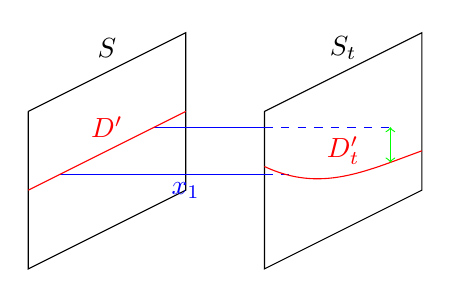
\begin{tikzpicture}
    \draw (0,2)--(0,0)--(2,1)--(2,3)--(0,2);
    \draw (3,2)--(3,0)--(5,1)--(5,3)--(3,2);
    \draw (1,2.8)node{$S$};
    \draw (4,2.8)node{$S_t$};
    
    \draw[blue] (0.4,1.2)--(3,1.2);
    \draw[blue,dashed] (3,1.2)--(3.4,1.2);
    \draw[blue] (1.6,1.8)--(3,1.8);
    \draw[blue,dashed] (3,1.8)--(4.6,1.8);
    \draw[blue] (2,1)node{$\pdiff{}{x_1}$};
    
    \draw[red] (0,1)--(2,2);
    \draw[red] (3,1.3) to [out=-25,in=200] (5,1.5);
    \draw[red] (1,1.8)node{$D'$};
    \draw[red] (4,1.5)node{$D'_t$};
    
    \draw[green][<->](4.6,1.8)--(4.6,1.35);
\end{tikzpicture}\]
    
    $[X_1,X_i]=\sum_{j=1}^c a_i^j X_j\ (i=2,\dots,c)$とすると、$l\geq c+1$に対して
    \[\pdiff{}{x_1}(X_i(x_l))=[X_1,X_l](x_l)=\sum_{j=2}^c a_i^j X_j(x_l)\]
    である、$X_1(x_l)=0$に注意。すると、これは$\{X_i(x_l)\}_i$という$c-1$個の未知変数についての線形常微分方程式をなし、$x_1=0$では初期値$0$を持つ($S$上では揃っている!)から$M$上で$X_i(x_l)=0$となる。つまり\\
    \[D_m\subset\set{v\in M_m}{\forall l\geq c+1\ v(x_l)=0}=\spn\left\{\pdiff{}{x_1},\dots,\pdiff{}{x_c}\right\}\]
    となるが、次元が等しいから上の包含は等号である。\\
    逆に、$\iota(P)\subset U$となる連結積分多様体$\iota:P\hookrightarrow M$について、$\iota(P)\subset\R^c\times\{{}^\exists a\}$となることを見る。それには$\pi:\R^d\to\R^{d-c}$について$\pi\circ\iota$が定数関数になればよく、その微分が消えるからOK。
    \[d(\pi\circ\iota)(P_p)=\pi(d\iota(P_p))=\pi(D_{\iota(p)})=0\]
\end{proof}


\ \\
\subsection{極大積分多様体}
\begin{lem}[積分多様体の位相]
    $\iota:P\hookrightarrow M$を$D$の積分多様体とする。このとき定理\ref{thm:123}でのスライス$S_a$について、任意の$U,a$に対し$\iota^{-1}(S_a)\subset P$が開になる。また、$\iota:\iota^{-1}(S_a)\to S_a\cap\iota(P)$は同相になる。
\end{lem}
\begin{proof}
    $p\in P$と$m:=\iota(p)$の近傍$U_p,U_m$を$\iota(U_p)\subset U_m$かつ$U_p$が連結となるように取る。$\iota:U_p\hookrightarrow M$も積分多様体だから、$\exists a\ \iota(U_p)\subset S_a$となる。つまり、$a\in\R^{d-c}$に対し$\iota^{-1}(S_a)$は$\supset U_p$か$=\emptyset$となる。これが全ての$p\in P$について成り立つから$\iota^{-1}(S_a)$は開になる。同相性は$\iota:\iota^{-1}(S_a)\to S_a$が同じ次元のはめ込み($\Rightarrow$開写像)になるため。
\end{proof}

\begin{thm}[命題\ref{prop:111}を参照]\label{thm131}
    $\phi:N\to M$が$\phi(N)\subset\iota(P)$を満たすとき、$\phi_0:N\to P$は連続。従って$C^\infty$級。
    \[\begin{tikzcd}
        N\arrow[rd,"\exists \phi_0"']\arrow[r,"\phi"] &M\\
        & P\arrow[u,hook]
    \end{tikzcd}\]
\end{thm}
\begin{proof}
    先の補題とほぼ同様である。$p:=\phi_0(n),m:=\iota(p),\ \phi(U_n)\subset U_m$と十分小さく近傍を取る。$U_n$を予め連結にしておく。$U_m\cap\iota(P)$の連結成分の個数は第二可算性から高々可算であり、各成分はあるスライスに入るから、結局$U_m\cap\iota(P)$は可算枚のスライスに含まれる。$\phi(U_n)\subset U_m\cap\iota(P)$は連結部分集合だから、$\phi(U_n)$はあるスライス$S_a$に含まれる。$\phi_0(U_n)\subset\iota^{-1}(S_a)$であり、前補題から$\iota^{-1}(S_a)\cap U_m$は$p$の近傍系をなすから$\phi_0$は$n$で連続。
\end{proof}
\begin{thm}[極大積分多様体]
    $D$を包含的とすると、$\forall m\in M$に対し$m$を通る極大積分多様体$\iota:P\hookrightarrow M$が存在する。つまり、$P$は連結であり、$\iota':P'\hookrightarrow M$を$m$を通る連結な積分多様体とすると$\iota'(P')\subset\iota(P)$となる(最大性)。
\end{thm}
\begin{proof}
    次は、「$U\subset M$が開$\overset{def}{\iff}\forall i\ \tau_i(U\cap U_i)\subset\R^n$が開」で位相が定まると思えばよい。このとき、$\tau_i:U_i\to\R^n$が同相になることを確かめればよい($U_i$には$M$からの相対位相が入っている)。
    \begin{rem}[多様体の定義]
        集合$M$を被覆する部分集合族$\{U_i\}_i$と全単射の族$\tau_i:U_i\to\R^n$が与えられたとき、次の条件を満たせば$M$は$\{\tau_i:U_i\to\R^n\}$をアトラスとする多様体構造が定まる。
        \begin{itemize}
            \item $\tau_j(U_i\cap U_j)$は開集合かつ、$\tau_j\circ\tau_i^{-1}:\tau_i(U_i\cap U_j)\to\tau_j(U_i\cap U_j)$は$C^\infty$級。
        \end{itemize}
    \end{rem}
    多様体$\Tilde{M}$を、集合としては$M$だが、アトラスとして次の写像の族$\{\tau_i:U_i\to\R^c\}$を持つものとする。
    \[\tau_i:U_i:=\tau^{-1}(\R^c\times\{a\})\overset{\tau}{\longrightarrow}\R^d\twoheadrightarrow\R^c\]
    ただし記号は定理\ref{thm:123}の通りであり、上の写像は可能な全ての$(U,\tau),a$で考える。これが上の注意の条件を満たすことを確かめる。$\tau_i(U_i\cap U_j)$が開であれば残りは自動的である。なぜなら、まず$U_i$は$\tau_i$を座標に持つ$M$の部分多様体であり、$\tau_i(U_i\cap U_j)$が開だから$U_i\cap U_j$も部分多様体になる。二つの座標$\tau_i,\tau_j$の座標変換は当然$C^\infty$級となる。\\
    今、$U_i=\tau^{-1}(\R^c\times\{a\}),\ U_j=\tau'^{-1}(\R^c\times\{a'\})$と、$(U,\tau,a)$と$(U',\tau',a')$から作られているとする。$U_j$は$D$の積分多様体だから$U\cap U_j$の各連結成分は$\tau^{-1}(\R^c\cap\{a"\})$という形の部分集合にスッポリ入っている。$U\cap U_j$の連結成分は$U_j$内で開だから、その合併である$U_i\cap U_j$も$U_j$内で開。$\tau_j$は同相だから$\tau_j(U_i\cap U_j)\subset\R^n$も開。\\
    \ \\
    上で作った$\Tilde{M}$での$m$の連結成分$P$には$\Tilde{M}$からの多様体構造が入る。示すべきは二つである:$P$の第二可算性と最大性。後者の方が簡単なのでそっちから片す。\\
    $\iota':P'\hookrightarrow M$を積分多様体とすると、$\iota':P'\hookrightarrow \Tilde{M}$も連続になる。これは$\iota'^{-1}(S_a)\subset P$が開であることから従う。故に$\iota'(P')\subset\Tilde{M}$は連結であり、$\iota'(P)\subset P$となる。\\
    $\Tilde{M}$のアトラスとして与えた$\{U_i\}$が「$\forall i\ \abs{\set{j}{U_j\cap U_i\neq\emptyset}}\leq\abs{\N}$」を満たすことを見ればいい。なぜなら「交わるかどうか」で添字集合にグラフ構造が入るが、各頂点の次数は高々可算だからグラフの各連結成分の頂点数も高々可算となり、グラフの連結成分への分解に応じて$\Tilde{M}$も開集合の非交和に分解される。つまり$P$が高々可算枚のアトラスで覆えることになり第二可算性が従う。\\
    $U_i$は全ての$(U,\tau),a$について考えると書いたが、少し変えて、$M$の第二可算性から$(U,\tau)$は可算枚で事足りるのでそうする。$U_i=\tau^{-1}(\R^c\times\{a\}),U_j=\tau'^{-1}(\R^c\times\{a'\})$と書くと、$U_i\cap U'$の連結成分は高々可算個だから、各$U'$について$U_i\cap U_j\neq\emptyset$となる$a'$も高々可算個の可能性しかない。可算×可算で$j$も高々可算個。
\end{proof}

\subsection{Cartanの方法}
$M,N$を多様体とする。各点$(m,n)\in M\times N$に対し、$\phi_{m,n}:M_m\to N_n$という線形写像の族が$m,n$に対し滑らかに与えられたとする。このとき、$\phi:M\to N$であって$\forall m\in M\ d\phi_m=\phi_{m,\phi(m)}$となるものが存在するか?という問が考えられる。
\[D_{(m,n)}:=\phi_{m,n}\text{のグラフ}:=\set{(v,\phi_{m,n}v)}{v\in M_m}\]
という分布がもし包合的ならば、Frobeniusの定理から極大積分多様体$\iota:P\hookrightarrow M\times N$が存在し
\[d\iota(P_p)=\phi_{\iota(p)}\text{のグラフ}\]
となる。故に、$P\hookrightarrow M\times N\to M$は同じ次元の多様体の間のはめ込みである。特に局所微分同相であり、つまり局所的には所望の写像$\phi:M\to N$が存在することになる。